\section{EXPERIMENTAL RESULTS}
\label{sec:exp}
The proposed framework for aging tolerance is implemented in C++ and the SAT-based formulation is solved by MiniSat on a 2.83GHz Intel Quad-Core CPU workstation running Linux. The benchmark circuits are chosen from the IWLS'05 and ISCAS'89 suites. The technology used is TSMC 45nm GP standard cell series.

Under 10-year BTI, the aging rates of clock buffers were obtained from HSPICE. The aging rates of clock buffers with duty cycles of 20\%, 40\%, 50\%, and 80\% are 8.51\%, 12.08\%, 13.51\%, and 16.41\% respectively and the aging rate of logic is obtained by using the predictive model presented in~\cite{wang2010impact},~\cite{wang2007efficient} (as in Section~\ref{subsec:apm}).

\begin{table*}
\centering
\caption{Results of aging tolerance}
	\begin{tabular}{l}
	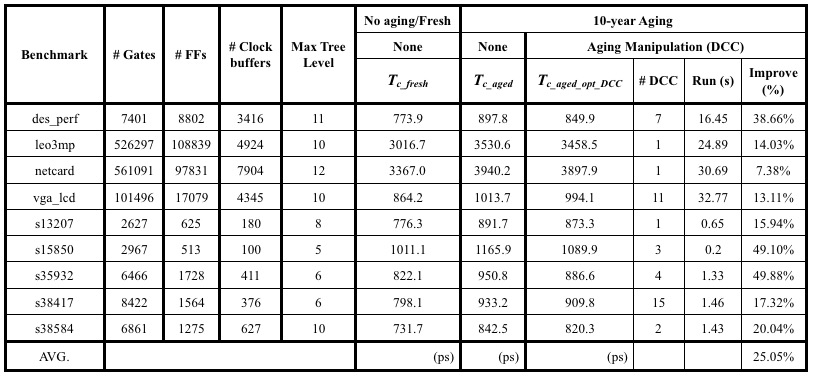
\includegraphics[width=1.3\columnwidth]{Experimental_result_(CG).png}
	\end{tabular}
\label{table:exp1}
\end{table*}
%\begin{table}[!t]
%\centering
%\caption{DCC insertion versus buffer insertion}
%	\begin{tabular}{c}
%	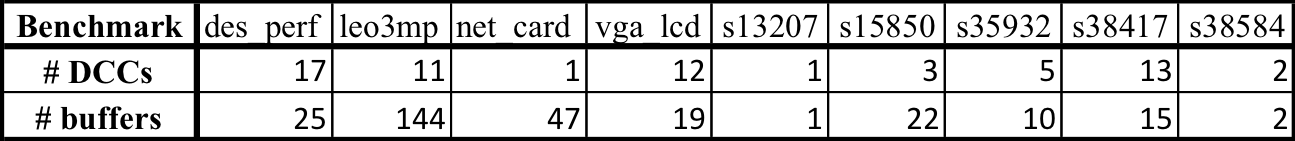
\includegraphics[width=0.8\columnwidth]{DCC_vs_buffer.png}
%	\end{tabular}
%\label{table:exp2}
%\end{table}

Table~\ref{table:exp1} reports the experimental results and information of each benchmark. Columns 2 to 5 show the total number of gates, total numbers of flip-flops, total numbers of clock buffers, and maximum level of the clock tree in each benchmark respectively. Column 6 demonstrates the fresh clock period that is the circuit delay without aging, denoted by $T_{c\_fresh}$. Column seven demonstrates the clock period of the circuit under 10-year aging, denoted by $T_{c\_aged}$. Column eight demonstrates the optimum clock period of the circuit under 10-year aging after applying our framework, denoted by $T_{c\_aged\_opt_DCC}$. Column 9 demonstrates the used DCC count. A shorter clock period under aging implies better circuit performance and higher level of aging tolerance. Column 10 demonstrates the runtime and the last column demonstrates the improvement, i.e., the level of aging tolerance which is calculated as:
\begin{gather*}
1 - (T_{c\_aged\_opt_DCC} - T_{c\_fresh}) / (T_{c\_aged} - T_{c\_fresh})
\end{gather*}

For benchmark \textit{des\_perf}, $T_{c\_fresh}$ is 773.9ps and $T_{c\_aged}$ is 897.8ps, which means after 10-year aging the clock period of circuit will increase by 123.9ps. With DCC insertion using the proposed framework, the clock period achieved is 849.9ps, an increment of 76ps against $T_{c\_fresh}$ (38.66\% improvement). As shown in Table~\ref{table:exp1}, the improvement ranges from 7.38\% to 49.88\% and is 25.05\% on average. \iffalse As shown in Table~\ref{table:exp2}.\fi The number of inserted DCCs is between 2 (for benchmark \textit{s38584}) to 17 (for benchmark \textit{des\_perf}), implying very limited degree of circuit modification and insignificant design overhead.

%\begin{figure}
%    \centering
%    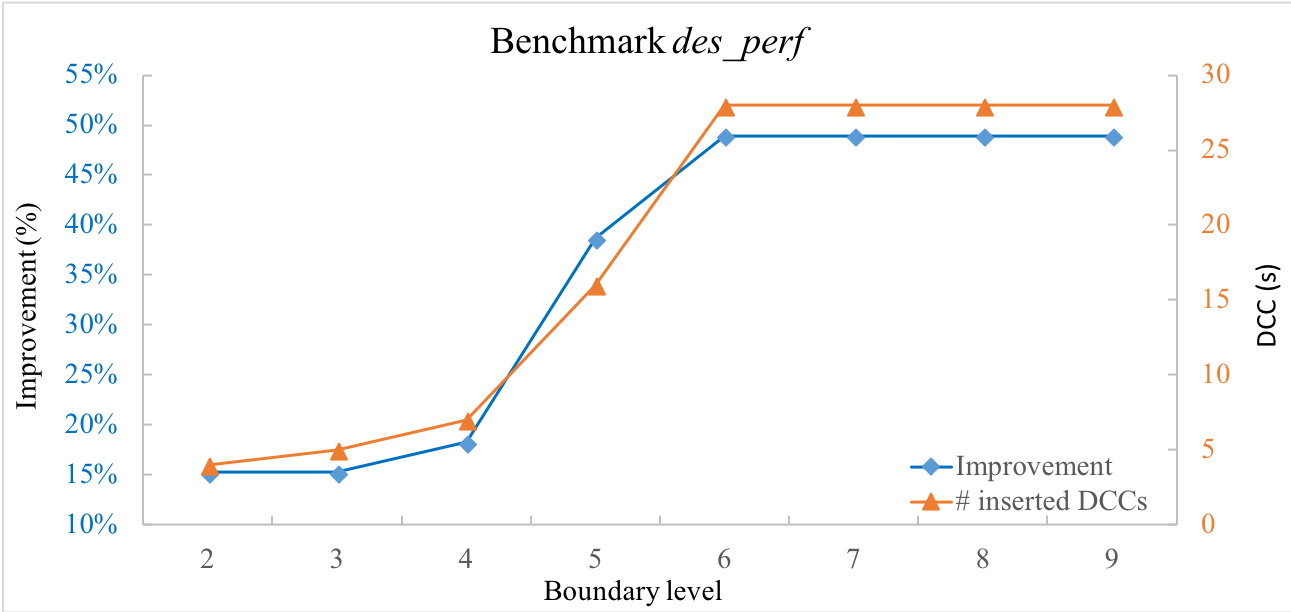
\includegraphics[width=0.8\columnwidth]{Boundary_level_vs_improvement.png}
%    \caption{Improvement/cost versus clock level considered}
 %   \label{fig:exp3}
%\end{figure}
%As mentioned in Section~\ref{sec:framework}, inserting DCCs deep in the clock tree is less effective. For benchmark \textit{des\_perf}, we considered the deployment of DCCs on the upper half of the clock tree (i.e., levels 1 to 5) and achieved 38.66\% improvement. As demonstrated in Figure~\ref{fig:exp3}, if we expand the boundary of DCC deployment from level 1 in the clock tree to level 6 and further up to level 10 progressively, we cannot gain much more improvement; however, more DCCs are required.

%For comparison purpose, we also apply buffer insertion to achieve the same $T_{c\_aged\_opt}$ in all post-CTS benchmarks. As it can be seen in Table~\ref{table:exp2}, the numbers of inserted DCCs are less than the numbers of inserted buffers in general. To achieve the same level of aging tolerance, we can expect our methodology based on DCC insertion to be much more cost-effective than buffer insertion.

\begin{figure}
    \centering
    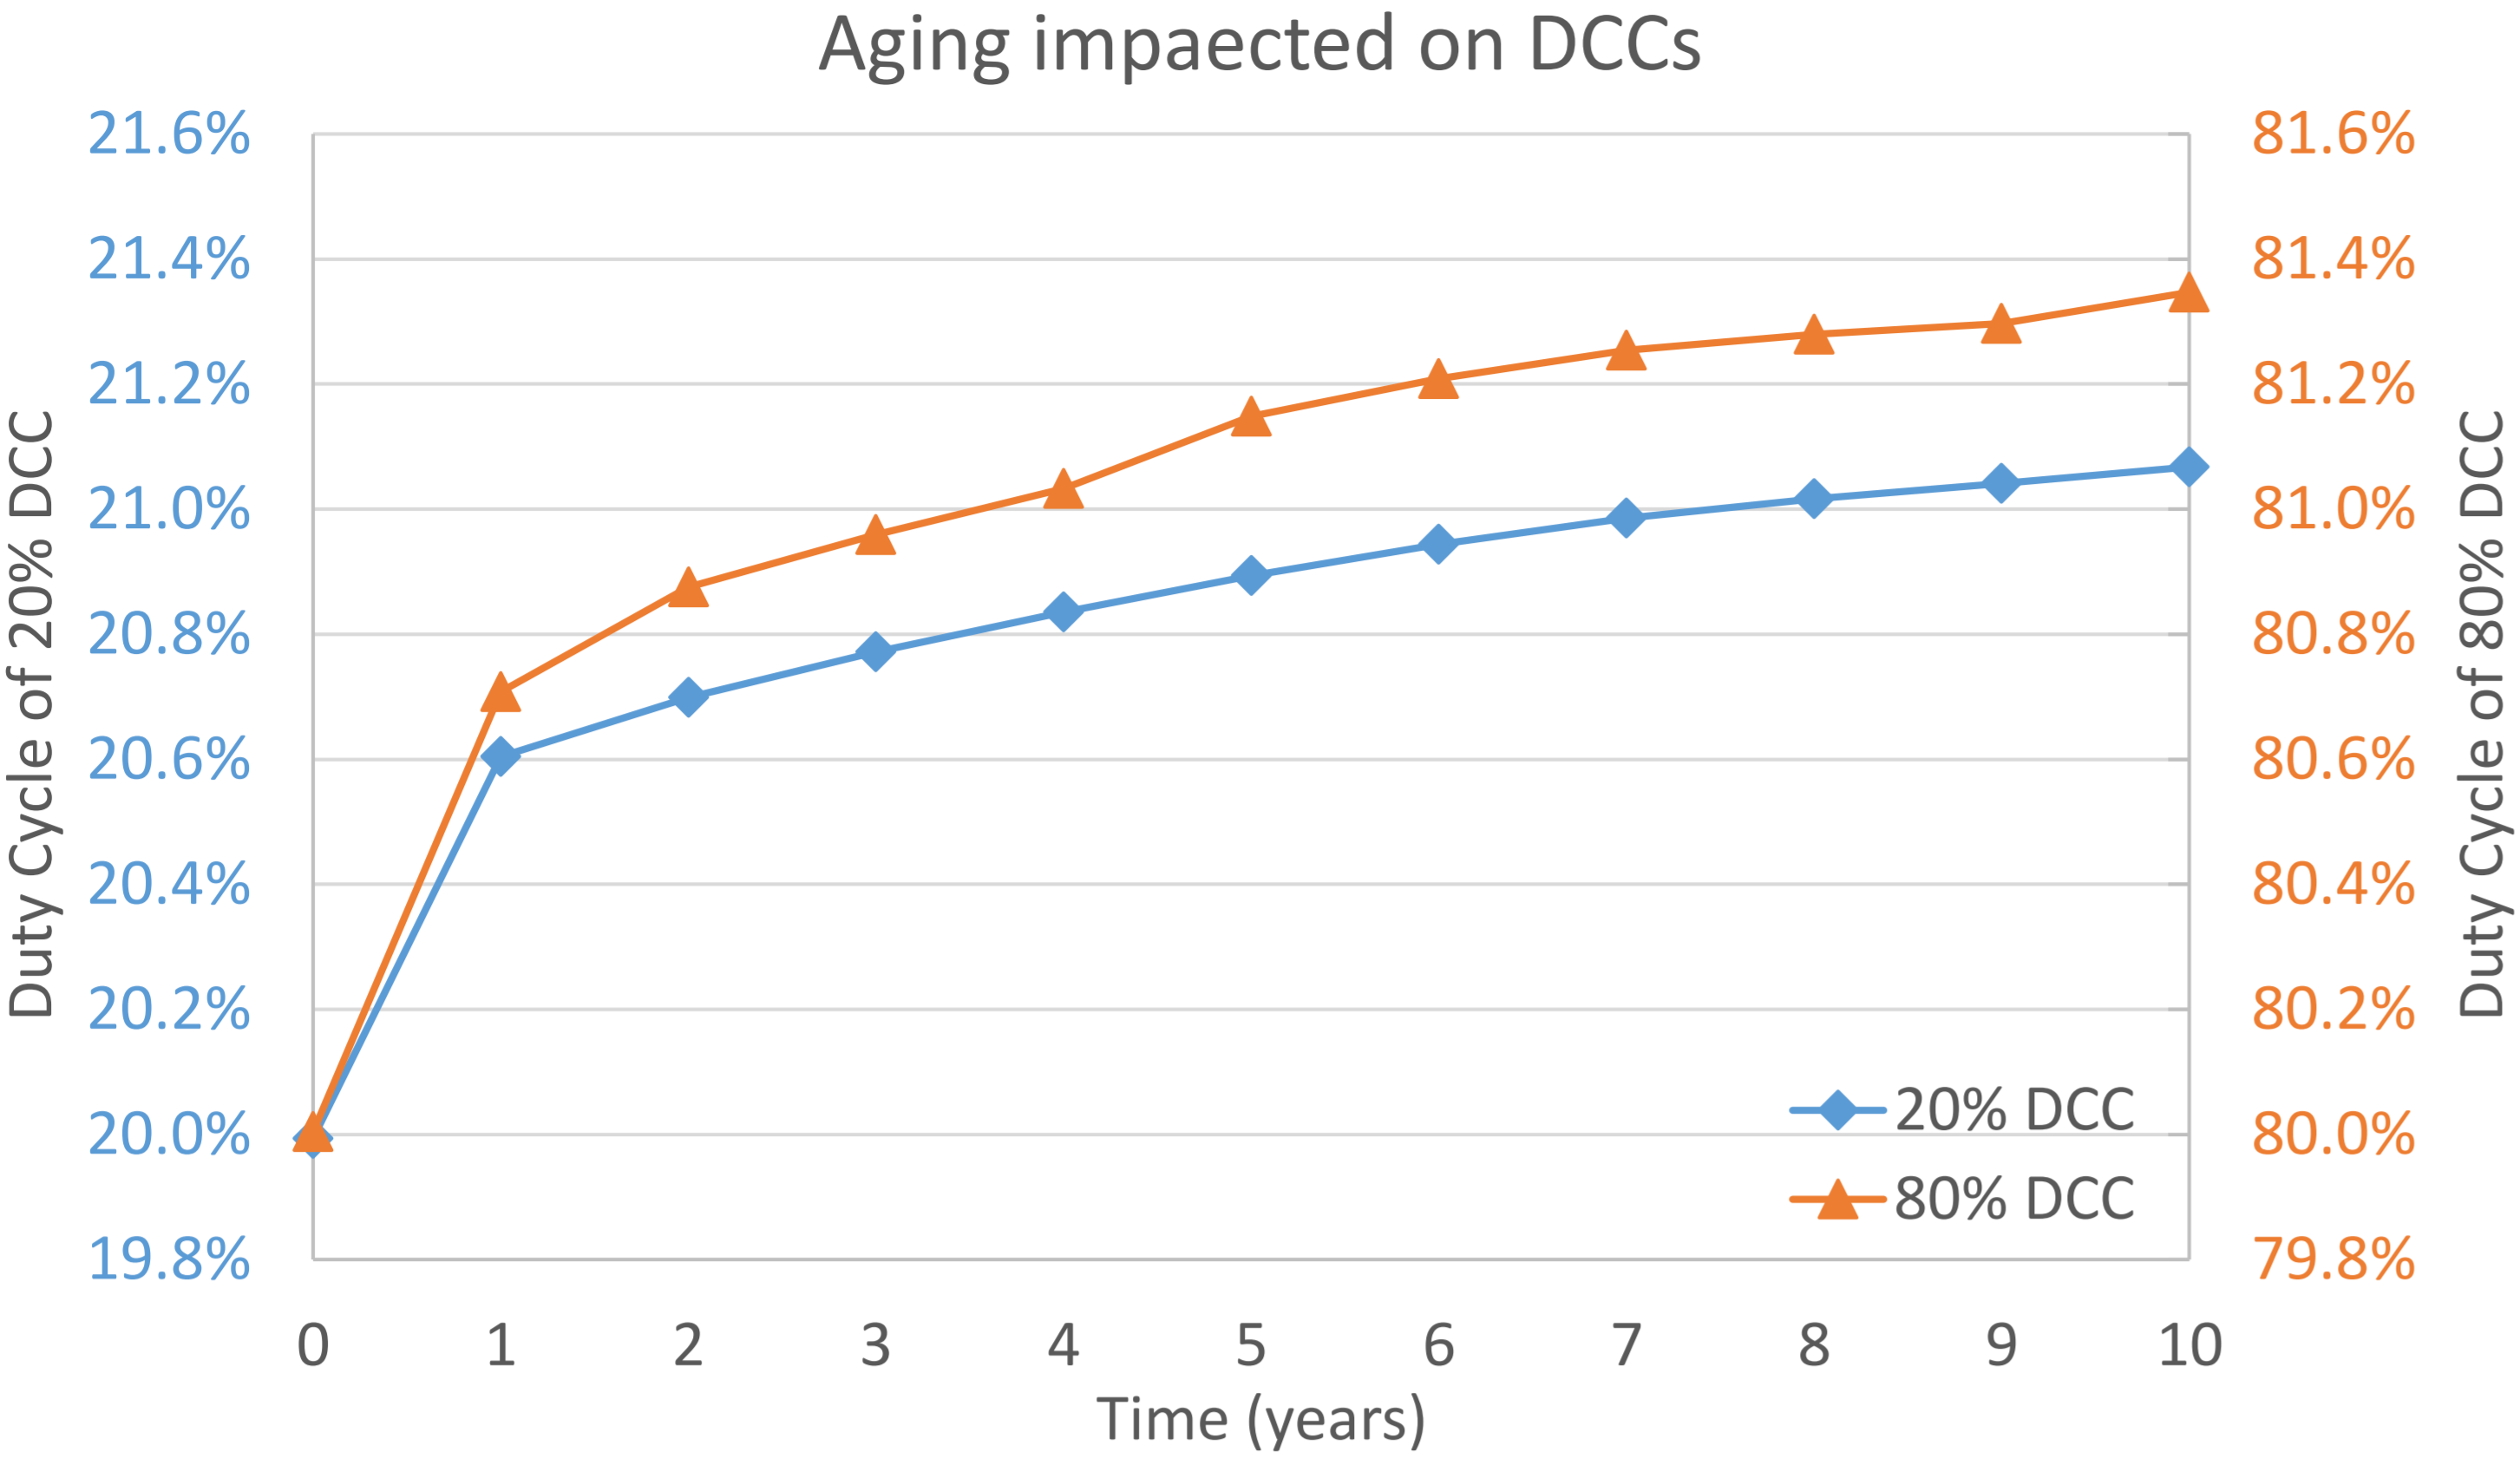
\includegraphics[width=0.8\columnwidth]{Aging_impacted_on_DCC.png}
    \caption{Aging impact on 20\%/80\% DCC under BTI}
    \label{fig:exp4}
\end{figure}

Figure~\ref{fig:exp4} shows the change in the duty cycle of a 20\%/80\% DCC over 10-year aging. The y axis on the left represents the duty cycle of a 20\% DCC, and the one on the right represents the duty cycle of an 80\% DCC. As it can be seen, the growth in both cases are marginal: $20\% \to 21.07\%$ for a 20\% DCC and $80\% \to 81.35\%$ for an 80\% DCC, which in turn should not affect the benefit of our proposed framework significantly.